

\begin{equation}
    cos(\theta) = \frac{
    \overrightarrow{v_1} \cdot \overrightarrow{v_2}
    }
    {
    \lvert\lvert\overrightarrow{v_1}\rvert\rvert
    \cdot
    \lvert\lvert\overrightarrow{v_2}\rvert\rvert
    }
    = w(e_i) \in G_{static}
\end{equation}

\subsubsection{Features and viewpoints}
\citeauthor{al2021microservice} \cite{al2021microservice} proposed a novel approach for the microservice identification based code embeddings. Code embeddings are similar to word embeddings and are able to capture the semantics of a code fragment. The technique first extracts methods from classes in the source code of the monolith, and subsequently converts them to code embeddings using the code2vec model created by \citeauthor{alon2019code2vec} \cite{alon2019code2vec}. The code2vec model represents the source code as a bag of Abstract Syntax Tree (AST) paths. The final clusters, obtained by applying the Affinity Propagation algorithm on the code embeddings, are evaluated by two microservice metrics introduced by \citeauthor{jin2018functionality} \cite{jin2018functionality}: Cohesion at Message Level (CHM) and Cohesion at Domain Level (CHD). The overall results of the decomposition appeared to outperform two similar approaches of \citeauthor{jin2018functionality} \cite{jin2018functionality} and \citeauthor{saidani2019towards} \cite{saidani2019towards}. \par
\citeauthor{de2018function} \cite{de2018function} proposed an approach that makes use of structural and behavioural properties of the system. The structural dependencies are discovered by looking at Create-Read-Update-Delete (CRUD) operations that represent the relation between database tables. The behaviour of the system is derived from log files and represented in a set of execution call graphs. These call graph are analysed to identify Frequent Execution Patterns (FEP). The approach is validated on an industry and open-source project by comparing the system's scalability, availability and efficiency of the old and new architecture. \par
\citeauthor{eski2018automatic} \cite{eski2018automatic} not only analyses structural dependencies but also captures code changes. They use static analysis over the source code to parse Abstract Syntax Trees (AST) and apply evolutionary analysis over the repository to detect changes between two consecutive commits in a Version Control System (VCS). The two are combined together in a software relation graph on which the Fast Community graph clustering is employed. This clustering is focused on maximizing the modularity function.
\par
\citeauthor{jin2018functionality} \cite{jin2018functionality} introduces one of the few methods that only relies on dynamic information of the system. They use two types of log traces: method-level and class-level execution traces. A method-level log trace presents the method-calling relation and invocation order. The class-level log trace shows which classes dedicate to the same functional execution. The method tend to cluster classes together that dedicate to the same business logic and thereby follows the 'Single Responsibility" microservice design principle.


To distinguishes software clustering approaches it is necessary to identify characteristics. Mitchell \cite{mitchell2003heuristic} defines the following characteristics:
\begin{itemize}
    \item \textbf{Degree of interaction.} There are three degrees of automation: fully-automatic, semi-automatic and manual approaches.
    \item \textbf{Deterministic or probabilistic}. In deterministic approaches the data that is used for the clustering is known beforehand and therefore will always produce the same result for a given input. In contrary, a probabilistic approach involves some elements of randomness and therefore may produce different outcomes given the same input.
    \item \textbf{Ability to cluster large systems.} Clustering large systems is computational expensive, and therefore the performance of the algorithm is important.
    \item \textbf{Distribution and accessibility of the tool.} How accessible is the clustering tool for interested researchers, students, and software engineers.
\end{itemize}

According to Mitchell \cite{mitchell2003heuristic}, software clustering approaches can be classified into the following categories: bottom-up, top-bottom, data mining and concept analysis techniques. 

Today's fast changing world requires companies to be flexible. To illustrate this, think about the current Corona pandemic that has increased (temporary) the activity on online web-shops. To handle this increased activity, it might be necessary to include extra server capacity. The microservices paradigm has gained more attention in the past years. 

Software maintainability and understandability is a daunting task when applications become larger. Therefore, experts could be helped by automated software clustering techniques. Depending on the purpose of the clustering, a clustering of software components will help to better understand the complexity of the application. Several software clustering techniques exists in the literature. They differ from each other in terms of different similarity measures, evaluation metrics, and data sources used (more?). \par
Software clustering is also used for service identification when migrating legacy systems to Service-Oriented Architectures (SOAs). Thus, there are roughly two main purposes of software clustering: (1) software clustering for \textbf{maintenance and recovery of software system structures} and (2) software clustering for \textbf{service identification} in order to migrate to a more modern architecture.

To validate the approach we will conduct a case study. The case study is performed on open source software that is freely available on the internet. Some examples of open source software that can be used in this thesis:
\begin{itemize}
    \item \href{https://app.diagrams.net/}{Draw.io}, a diagramming application. The software is available as web application and desktop application. The web app is mainly written in JavaScript and the desktop application in Java. The software is published on Github and can be find by this link: \href{https://github.com/jgraph/drawio}{https://github.com/jgraph/drawio}. An advantages of Draw.io is that there is a default log4j configuration implemented for the desktop application. This could save time. 
    \item JabRef is a desktop application for managing BibTeX and biblatex (.bib) databases written in Java. The software is open sourced and accessible by this link: \href{https://github.com/JabRef/jabref}{https://github.com/JabRef/jabref}.
\end{itemize}

This \href{https://github.com/davidetaibi/Microservices_Project_List/blob/master/README.md}{Github page} gives you a curated list of Open Source projects developed with a microservices architectural style.


% ----------
% CLUSTERING
% ----------

\citeauthor{wiggerts1997using} \cite{wiggerts1997using} divides software clustering algorithms in roughly four categories: (1) graph theoretical algorithms, (2) construction algorithms, (3) optimisation algorithms, and (4) hierarchical algorithms. We will describe each category shortly. \citeauthor{alsarhan2020software} \cite{alsarhan2020software} discriminates between \textit{hard and soft clustering} where in hard clustering software entities can only exist in exactly one clustering while in soft clustering this is not a hard constraint. In other words, this means that hard clustering must produce disjoint clusters while in soft clustering there might exist overlapping. Within hard clustering, we divide two type of algorithms: hierarchical and partitioning clustering. 

Clustering can also be seen as an optimisation problem in which we aim to find the global optimum. In general, optimisation algorithms take an initial partitioning and try to improve it by iteratively making adaptations according to some heuristics \cite{wiggerts1997using}. Below we discuss two optimisation techniques.

\paragraph{Simulated Annealing}
Simulated annealing is a probabilistic optimisation algorithm proposed by \citeauthor{kirkpatrick1983optimization} \cite{kirkpatrick1983optimization} in 1983 for approximating the global optimum of a given function.  

% -------------------
% SOFTWARE CLUSTERING
% -------------------

However, the clustering objective influences the result of the clustering. In the literature, we have observed the following categories of software clustering techniques. The division is driven by the granularity level they consider in the clustering. 

\subsubsection{High-level software clustering}
In high-level software clustering, the obtained clusters represent high-level component abstractions of the system \cite{saeidi2015search}. This is also called file level clustering. File clustering helps the programmer to better understand and maintain complex software. The result of the clustering represents a high-level view of the system.  \citeauthor{saeidi2015search} \cite{saeidi2015search} performs high-level software clustering by extracting dependencies between modules (files) and calculating the semantic similarity of files. The semantic similarity of a file is calculated by looking at identifier names and comments embedded in the source code. \citeauthor{anquetil1998extracting} \cite{anquetil1998extracting} shows that file names are a good criterion for high-level software clustering. Most of the techniques related to software clustering use lower-level information of the system. These are discussed in the next section.

\subsubsection{Low-level software clustering}
In order to identify services, it is important to also look at lower-level data. 

Decomposition techniques are not only used for deriving suitable microservices. Back in the days, decomposition techniques were mostly used to gain better understanding of software. However, the decomposition did not result in fine-grained services, but rather in more abstract software boundaries. Therefore, this process is rather called software clustering. 

Decomposing the monolith has many similarities with software clustering. 
The software clustering problem is defined as grouping closely related nodes into clusters, where nodes are represented as the system's modules (e.g. files, classes) \cite{Doval1999}. Most of the research that tries to cluster subsystems represents the structure of a software system as a directed graph \cite{mitchell2003heuristic}. This graph that represents the structure of a system is called a Module Dependency Graph (MDG) according to Doval et al. \cite{Doval1999}. A cluster of software components that are highly inter-dependent is also called a partition. 

Many times, MDG's are used as input for a clustering algortihm. The cluster algorithm searches through the solution space to select the most optimal partition of the MDG. A good decomposition, or partition, is defined by (1):
\begin{itemize}
    \item \textbf{Low number of inter-cluster relationships.} The connectivity between clusters. A low number of inter-cluster relationships is desired because it indicates that two clusters are largely independent.
    \item \textbf{High number of intra-cluster relationships.} The density of connections between nodes inside a single cluster. This means the modules are highly dependent from each other.
\end{itemize}

However, comparing software clustering to microservice identification, we notice that the two differ in the information and objective metrics they consume.
+TODO

% -------------
% MICROSERVICES
% -------------

Most of the approaches are built around microservices principles. This means that the decomposition result depends on the microservice principles. Therefore, it is important to understand which principles are present in the literature.

"Newman advocates thinking of microservices as a particular approach for SOA (Service-Oriented Architecture) and also defines microservices by seven principles, including “Model around business concepts”, “Decentralize all the things”, “Make ser- vices independently deployable”."

"Richardson [10] provided four decomposition strategies, i.e. “decompose by business capability”, “Decom- pose by domain-driven design sub domain”, “Decompose by verb or use case” and “Decompose by nouns or resources”. "

\citeauthor{selmadji2018re} \cite{selmadji2018re} describes four microservice principles.

\citeauthor{lohnertz2020steinmetz} \cite{lohnertz2020steinmetz} uses two principle, namely: each service should have independent software life cycles (seperation of teams). And one service should only have one task, the single responsibility principle.

\cite{gysel2016service} uses Domain-Driven-Design to obtain service boundaries.

\citeauthor{nunes2019monolith} \cite{nunes2019monolith} states that the microservice principles that are used to dictate the decomposition are strongly related with the type of information that is collected.

+TODO

% ---------------------
% DECOMPOSITION QUALITY
% ---------------------

\subsection{The quality of a decomposition}\label{ss:quality_decomposition}
There are several ways to measure the quality of a microservice decomposition. One of the most popular approach is to compare the automatically obtained decomposition with a golden standard. A golden standard in this case is a decomposition derived manually from experts. 
+TODO


% -----------------
% PROBLEM STATEMENT
% -----------------

\subsubsection{Scientific contribution}

\subsubsection{Company relevance}
In practice, companies do not always have the information that is necessary in place. It could happen that log files are missing, or that the identifier names in the code are anonymised. Many approaches only rely on a single source of information, but what if that source is missing. How does it affect the quality of the decomposition? 

% ----------------------
% TO BE USED, CLUSTERING
% ----------------------

\subsubsection{Comparison of algorithms}
Genetic algorithms are typically used in large search spaces in which finding solutions brute-force is not feasible in the context of time. 

An advantage of genetic algorithms is that they perform globalised search for solutions whereas most clustering procedures perform a localised search \cite{rokach2005clustering}. In a localised search, the solution in the next iteration is close to the current solution, and therefore may stop earlier in sub-optimal solutions. K-means and fuzzy clustering algorithms are examples of localised search algorithms \cite{rokach2005clustering}. GAs produce new solutions that can be completely different from the current ones and therefore are less prone to get stuck at the local optimum.
Moreover, genetic algorithms are less sensitive to the initial cluster centres (k-means).

Several papers have used GAs for the task of identifying software boundaries \cite{saeidi2015search} \cite{Doval1999} \cite{saidani2019towards} \cite{zhang2020automated}. 
+TODO


% -----------------------------------
% OLD RELATED WORK SECTION
% -----------------------------------

%\subsubsection{Decomposition methods}
%After obtaining the correct data, we have to choose an algorithm that identifies microservices. We have found two type of techniques that are commonly used: clustering algorithms and search-based genetic algorithms. The two are discussed below.

%\paragraph{Clustering algorithms}
%Most of the analysed decomposition approaches make use of an clustering algorithm. A clustering algorithm groups objects in such a way that objects in the same group are more similar to each other than objects in other groups. We notice that the hierarchical clustering algorithm is the most popular algorithm as it is used in \cite{jin2018functionality} \cite{matias2020determining} \cite{nunes2019monolith} \cite{ren2018migrating} \cite{selmadji2018re} \cite{selmadji2020monolithic}. \citeauthor{ren2018migrating} \cite{ren2018migrating} combined hierarchical clustering with k-means clustering. The paper of \citeauthor{lohnertz2020steinmetz} \cite{lohnertz2020steinmetz} experimented with 7 different cluster algorithm and detected that the Louvain algorithm is performing the best among microservice identification.  

%\paragraph{Search-based genetic algorithms}
%Search-based genetic algorithms are less popular and are only used in two papers \cite{saidani2019towards} \cite{zhang2020automated} found in the literature review. Both approaches use the Non-dominated Sorting Genetic Algorithm II (NSGA-II) introduced by \citeauthor{deb2002fast} \cite{deb2002fast}. Genetic algorithms are search-based algorithms and allow microservice identification to be a multi-objective problem. This means that it is able to optimize multiple objective functions simultaneously. 

%\subsubsection{Validation types}
%The papers found in the literature show different ways of measuring the success of their result. The validation types can be divided into two groups: internal and external measures. The internal assessment refers to an intrinsic evaluation of the clustering results and relies on certain metrics. In an external assessment the obtained services are compared with an expert decomposition (authoritative decomposition) which has been obtained by manually inspecting the system, or with the results deriving from state-of-the-art techniques that are used on the same system. 

%\paragraph{External assessment: comparison to expert decomposition}
%The most popular validation type is an external assessment in which the results are compared to a golden standard \cite{eski2018automatic} \cite{kamimura2018extracting} \cite{nunes2019monolith} \cite{selmadji2018re} \cite{selmadji2020monolithic} \cite{zhang2020automated}. \citeauthor{eski2018automatic} \cite{eski2018automatic} used the MoJo similarity metric to measure how close the decomposition is to the authoritative decomposition. \citeauthor{kamimura2018extracting} \cite{kamimura2018extracting} validates their approach on the 'Spring Boot Pet Clinic' application that has both a monolith and microservice version. They match the results of the decomposition derived from the monolith version to the results of the microservice version and identify similarities and differences. \citeauthor{nunes2019monolith} \cite{nunes2019monolith} uses pairwise precision, recall and f-score to compare the generated decomposition with the expert decomposition. Also the method by \citeauthor{selmadji2018re} uses precision and recall to measure the quality of the decomposition. Their follow-up paper only uses the recall metric \cite{selmadji2020monolithic}. In both papers experts are asked to classify each microservice as excellent, good or bad. Having this knowledge, the precision expresses the ratio between good an excellent identified microservices to the total classified ones. Recall is the ratio between the number of good and excellent microservices to the number of manually identified ones.

%\paragraph{External assessment: comparison to state-of-the-art methods}
%Many approaches use the same test cases and thus are comparable with each other. For example, JPetstore\footnote{https://github.com/mybatis/jpetstore-6} and SpringBlog\footnote{https://github.com/Raysmond/SpringBlog} are two popular open-sourced applications written in Java that are used by \cite{al2021microservice} \cite{jin2018functionality} \cite{saidani2019towards}. This enables \citeauthor{al2021microservice} \cite{al2021microservice} to compare their results to the ones obtained by \citeauthor{jin2018functionality} \cite{jin2018functionality} and \citeauthor{saidani2019towards} \cite{saidani2019towards}. The results of \citeauthor{jin2018functionality} \cite{jin2018functionality} are also used for comparison in the work of \citeauthor{zhang2020automated} \cite{zhang2020automated}. \par
%The least popular validation approach is comparing the performance of the old architecture with the new architecture. This could be due to the fact that it causes many difficulties and obstacles since the decomposition is not only an illustration but actually used to migrate the system to the new microservice architecture. We have found two papers that follow this validation type. The first one, introduced by \citeauthor{de2018function} \cite{de2018function}, measures the impact of the decomposition by recording execution times, memory consumption and disk consumption. Based on these findings the scalability, availability and execution efficiency of the old and new system are calculated and compared to each other. \citeauthor{ren2018migrating} \cite{ren2018migrating} also measures the application performance under a monolithic and microservices architecture. They use the throughput and loads metric to compare the two architectures. 

%\paragraph{Internal assessment: microservice metrics}
%To measure the success of the decomposition method, it is important to understand what defines a microservice. There have been proposed several metrics that try to quantify the quality of a microservice. The work of \citeauthor{jin2018functionality} \cite{jin2018functionality} defines the quality metric \textit{functional independence} that quantifies the independence to which microservices present their own functionalities. The functional independence is measured by five metrics: cohesion at domain level (CHD), cohesion at message level (CHM), interface numbers (IFN), operation numbers (OPN), and interaction numbers (IRN). The CHD and CHM measure the functional cohesion of microservices while IFN, OPN and IRN measure the coupling between microservices. The functional metrics are also used in related studies \cite{al2021microservice} \cite{saidani2019towards}. \citeauthor{lohnertz2020steinmetz} \cite{lohnertz2020steinmetz} selected six metrics to evaluate the quality of the decomposition. The \textit{input fidelity} shows the percentage of classes that are covered by the given input. Next they use the \textit{number of clusters, number of inter-cluster edges, ratio of inter-cluster edge weights and mean cluster factor} to measure the general cluster quality. Lastly the \textit{modularity} metric proposed by \citeauthor{newman2004fast} \cite{newman2004fast} is included.


% -----------------------------------
% GOALS
% -----------------------------------

% MUST HAVES

%\item Select an appropriate target (monolithic) software system, preferably open sourced
%\item Find tools that help extracting data from software (e.g. static analysers, dynamic analysers). 
%\item Filter and preprocess the extracted data for example to remove unnecessary textual and nontextual information from comments and source codes.
%\item Identify the software entities that have to be clustered. The input entities depend on the abstraction level on which we aim to cluster.
%\item Merge the aforementioned data together into a two-dimensional feature matrix.
%\item Define a suitable similarity measure that represents the similarity between two entities based on their features.
%\item Select and run a clustering algorithm.
%\item Select a set of evaluation metrics to compare the results of the clustering.
%\item Compare the different clustering results and answer the research questions.

\section{Modelling microservices}

Let's formally encode the microservices problem. In Python, a program \textit{P} consists of modules \textit{M} that subsequently consists of classes \textit{C} and functions \textit{F}. A function can be defined inside a class, a function (called nested function) or at module level. In this thesis, we consider the union over the set of classes and functions as the set of code elements \textit{CE}. This is the finest level of detail where we want to cluster on. This means that a microservice \textit{M} is a partition of the set of code elements, such that there is a maximal degree of intra-connectivity and minimal degree of inter-connectivity. In other words, this means that code elements within a microservice should have high similarity while code elements between microservices should be dissimilar.\par

To make the definition more understandable, we apply it to our running example. We only use the modules Order and Orderdetail to keep it easy to understand. The Order module consists of the functions $create\_order()$ (CE$_{1}$) and $view\_orders()$ (CE$_2$) while the orderdetail module consists of the function $create\_orderdetail()$ (CE$_3$). This means that there are two modules M = $\{O, OD\}$ resulting in a total set of  code elements CE = $\{CE_1, CE_2, CE_3\}$.

A code element carries three sources of information. The first one considers the dependencies D. A dependency D between two code elements is defined as an invocation between them: D = $\{(code\_element, dependency)\}$. To illustrate, when the function $create\_orderdetail$ invocates the method $get\_product$, this is denoted as a dependency: $\{(create\_orderdetail, get\_customer)\}$.\par
A code element can be represented as a set of features F. As mentioned before, we consider three types of features in this research. The first one are dependencies D. The second one captures the semantic meaning and the third one focuses on the execution of the program.

\begin{lstlisting}[language=Python, caption=Python example]
class Orderdetail:
    def __init__(self, order_id, product_id, quantity):
        self.product = get_product(product_id)
        self.order = get_order(order_id)
        self.quantity = quantity
    
    def create_orderdetail(self):
        '''Create an orderdetail in the database.'''
        if Product.check_stock(self.quantity):
            if Order.exists(self.order_id):
                ...
\end{lstlisting}

\section{Running example}

To clarify thoughts throughout this research, we will use a simple running example. The running example shows the reader intuitively the workflow and expected outcome of the approach.

\subsection{Context description}
PyPetstore\footnote{https://github.com/larsvasseldonk/salie} is a very simple command-line tool written in Python that helps managing the process of selling pets. The application is inspired by JPetstore\footnote{https://github.com/mybatis/jpetstore-6}, a Java application that is often used in related papers to describe the working of their approach \cite{al2021microservice, jin2018functionality, jin2019service, saidani2019towards, zhang2020automated}. In PyPetstore, users are able to create orders, add products to it, manage the availability of products, and get an overview of its customer base. The data acquired by the application is save into a SQLite database that consists the following structure (see Figure \ref{fig:salie_ERD}). The application is implemented in seven modules, that each implements the following functionality.

\begin{enumerate}
    \item \textbf{Customer.} The customer module allows users to create, update, delete, view, and search for customers in the database.
    \item \textbf{Database.} The database module initialises the database and its corresponding tables and is responsible for the database connection.
    \item \textbf{Order.} The order module enables users to create, view and search for orders in the database.
    \item \textbf{Orderdetail.} The orderdetail module assures that products can be added to an order. It is able to create and view order details.
    \item \textbf{Product.} The product module manages the product entities in the database. The module is able to create, delete, view and search for products.
    \item \textbf{Util.} This module contains some utility functions like the menu printing function.
    \item \textbf{Main.} The main module holds the application together. The main implements the workflow of the application.
\end{enumerate}

\begin{figure}
    \centering
    \captionsetup{justification=centering ,margin=1.5cm, labelfont=bf, font=footnotesize}
    \caption{Entity Relationship Diagram (ERD) of the running example.}\label{fig:salie_ERD}
    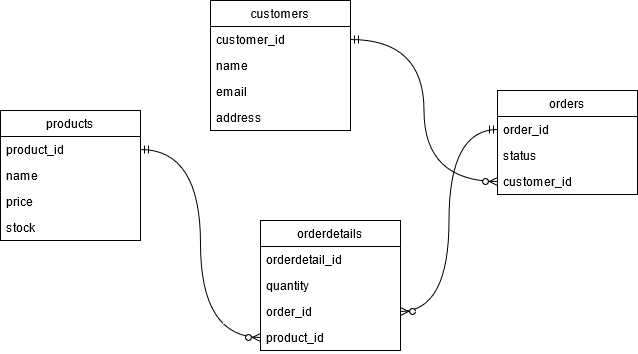
\includegraphics[scale=0.55]{figures/salie_ERD.png}
\end{figure}

The modules have certain dependencies. For example, to create order details, we need to have an order and a product. And to create an order, we need to have a customer.\par
Next, imagine that the architect wants to split up the application to get a more flexible architecture. As described in Section \ref{s:information_views}, there are several sources of information on which the architect can rely on. In this thesis, we focus on static dependencies, semantics, and dynamic information obtained from the system. This running example will be used throughout the thesis to clarify the approach.

\begin{table}[h]
    \footnotesize
    \captionsetup{justification=centering ,margin=1.5cm, labelfont=bf, font=footnotesize}
    \caption{Top 10 words belonging to each topic.}\label{tab:topic_distribution}
    \begin{tabular}{>{\raggedright}m{30pt}>{\raggedright\arraybackslash}m{282pt}}
        \toprule
        Topic 1
        & menu print sale finance get insights main function program module \\
        \midrule
        Topic 2
        & os table create conn sqlite connection error orderdetails close database\\
        \midrule
        Topic 3
        & order data product customer sql db search delete quantity stock\\
        \midrule
        Topic 4
        & status input conn customer sqlite connection choice error util create\\
        \midrule
        Topic 5
        & sale orderdetail email close connection name orderdetails database create manage\\
        \bottomrule
    \end{tabular}
\end{table}

% h = float specifier
% 312pt is the full-width of the table

To measure the quality of the decomposition, various microservice specific measures has been proposed. Many of those metric rely on the interfaces and its operations that are extracted from the system. To get a better understanding of what these terms mean, lets illustrate it in the running example. Assume that we have:

\begin{itemize}
    \item Module Order.py that contains the class Order. To initiate an Order object we need to have a customer. For this we use the method get\_customer() defined in the Customer class.
    \item Module Customer.py that contains the class Customer that implements the method get\_customer()
\end{itemize}

After decomposing the system in microservice, each class is partitioned into a separate service. However, to create an Order we still need to have use the function get\_customer() located in the Customer service. This because we do not duplicate methods. To let the service Order make use of the get\_customer() method, we need to define an \textit{interface}. In papers that cluster at Class granularity, an interface contains all the methods of the class that are invocated from outside the service. However, in this approach we tend to decompose the system at function/method level. This way, each interface consists of only one method or function.

An interface is a set of operations (functions that are defined inside a class) that can be accessed by other microservices. Therefore, when implementing, the operations in the interface should all be accessible via messaging communication by the outside world.

% --------------------
% DISCUSSION
% --------------------

%A higher IFN rate means bigger services and thus less external communication between services are necessary \cite{brito2021identification}. However, this is not reflected by the semantic obtained decompositions since they rather optimise CMQ then SMQ. When semantic information is included, the graph contains significantly more edges. In, e.g., the picard application, the number of edges increases from 570 for static information, to 21555 for semantic information. This is a big increase. This big increase of semantic edges occurs whenever semantic data is included. The high amount of the semantic edges can be reduced by varying the tf-idf threshold. \par

%\begin{itemize}
%    \item Table \ref{tab:results_ifn} shows that the number of interfaces (IFN) is much higher when semantic data streams are included. This means that only focusing on semantic data results in a higher amount of interfaces, which is undesirable.
%    \item The structural modularity quality (given in Table \ref{tab:results_smq}) of a decompositions purely made of semantic data is very low. When incorporating semantic information with static or dynamic information, we observe that the SMQ value (significantly decreases). This is also inline when observing the data given by \citeauthor{jin2019service} \cite{jin2019service}. In this paper, they compare their approach to the one proposed by \citeauthor{mazlami2017extraction} \cite{mazlami2017extraction}, which is called Microservice Extraction Model (MEM). In MEM, where the edges are constructed with only semantic information (logical and contributer information are left out due to their low coverage), the models shows a very poor performance in terms of SMQ value.
%    \item The best SMQ value is almost always achieved (5/6) when combining static and dynamic data with each other.
%    \item The number of operations (OPN) is much higher when semantic data is included. When comparing the single source experiments ($ex_1, ex_2, ex_3$), we see that the results in which only semantics are used result in a much higher rate of OPN.
%    \item Incorporating all streams of information sources ($ex_7$) never results in the best decomposition in terms of functional independence and modularity. The coverage, in contrary, has the highest value when incorporating multiple information sources. This makes sense since including different views ensures that more top-level code fragments of the system are touched.
%    \item There is not an obvious pattern when combining two information sources with each other. 
%    \item A higher OPN rate means more communication between services and thus results in a lower SMQ score. The lowest OPN score is achieved when only static data is included. However, the lowest SMQ rate is achieved when static and dynamic data is combined. This is because combining static and dynamic data results in a bigger IFN rate. A bigger IFN score means that more interfaces are included in less services. This then also means that the resulting services will be bigger, and bigger services result in less external communication and thus a higher SMQ rate.
%\end{itemize}

%Regarding the number of operations (OPN), we note that decompositions made with semantic data result in much more operations. A worse OPN score also results in a worse SMQ score. This makes sense since more operations means more external connections between services are made. 
%IFN represents the average number of interfaces services have. The higher this number, the more published interfaces a service contains. A high IFN rate means that services contain many interfaces on average. 
%A higher IFN score means that the service that communicate with other services have many external connections. 

%Before the execution of this experiment, we expected graphs that include multiple sources of information would result in a better decomposition than when less source of information are used. Following this expectation, we would assume that the best decomposition is achieved when all three sources of information are included ($ex_7$). However, the results of our experiment do not support this pattern. Out of the six metrics that measure the quality of microservice decompositions, none scores the highest when all informations streams are included. The only metric that performs the best when all information is included is the coverage. This makes sense since more data means that more aspects of the system are touched and thus clustered. \par
%One of the reasons for this could be the influence of the coverage. When more information is included, the coverage of decomposition increases which means that more nodes and connections are added.

%The main goal of this thesis is to find out the impact of multi-view clustering in the domain of microservices. The results in Chapter \ref{c:results} show the quality of each decomposition that is constructed with a different stream of information. This way, we can compare each stream of information with each other to find out what the impact of each individual source is. We try to make the results as generalisable as possible by, for example, testing the approach on input projects from different sizes and by cancelling out the effect of the clustering algorithm. For this reason, the results should also be applicable for decomposition made with different clustering algorithms. Even though we think the results are generalisable, we also have discovered some threats to validity.

%\subsubsection{Algorithms are independent of change in the results}
%As mentioned before, we cancel out the effect of the clustering algorithm by assuming that the change of the results is independent from the selected algorithm. This assumption is supported by data (see Table \ref{tab:effect_algorithm}) obtained from a small experiment where two projects are decomposed with four different algorithms. However, this experiment is not executed on a large scale and therefore there is a threat that the algorithm does have effect on the change in the results.

%\subsubsection{Test scenarios may not represent the real-world}
%We collect log information by running test scenario's that are available in the repository of the target project. However, these tests are mainly created to test the working of certain functionalities rather than simulate the behaviour of real-world users. Logs obtained with test scenario's show which functions invocates each other at runtime and their frequency, but do not reflect the behaviour of real world users. When log data is acquired by real users, we may see that some aspects of the system are are more frequently used together than others. We have to be aware that this user data is not reflected in our log files.

%\subsubsection{Frequency in static analysis not considered}
%Unfortunately, PyCG does not consider the frequency of structural dependencies. Thus when function $X$ uses function $Y$ three times, only a single dependency will be covered.